
%-------------------------------------------------------------------------%
\section{The Standard Model}
The standard model (SM) describes the interaction of the three fundamental forces (electromagnetism, strong, and weak forces) with matter, where each force is described by a corresponding Quantum Field Theory (QFT). It is understood that these forces have developed a building block with three generations of fundamental particles called \textit{fermions} in quarks and leptons, categorized by its half-integer spin. For quarks, we have \textit{up}, \textit{down}, \textit{charm}, \textit{strange}, \textit{top}, and \textit{bottom} \cite{griffiths2008introduction}. The quarks exist in a bound state known as \textit{hadrons} and can never be observed directly \cite{thomson2013modern}. For leptons, we have \textit{electrons}, \textit{muons} and \textit{taus} that have mass, with their associated \textit{neutrinos} that are massless according to observations  (See Table \ref{tab:SMFerm}) \cite{griffiths2008introduction}. In association with each particle, there exists its anti-matter (denoted with a bar above i.e. $\Bar{particle}$).  The number of particles seen in Table \ref{tab:SMFerm} may also be doubled when we consider the chirality of the particles i.e. if it is right-handed or left-handed. This can be an important aspect in studying particle interactions as the interactions moderately differ between the right- and left-handed particles. \\

\begin{table}[htbp]
    \centering
    \begin{tabular}{||c|c|c|c||}
    \hline
    & Gen1 & Gen2 & Gen3 \\
    \hline
    \multirow{2}{1.2cm}{quarks} & $u$ & $c$ & $t$ \\
     & $d$ & $s$ & $b$ \\
    \hline
    \multirow{2}{1.2cm}{leptons} & $e$ & $\mu$ & $\tau$ \\
     & $\nu_e$ & $\nu_\mu$ & $\nu_\tau$ \\
    \hline
    \end{tabular}
    \caption{The three generation of fermionic matter in the Standard Model.}
    \label{tab:SMFerm}
\end{table}

The first generation of elementary particles (electron, electron neutrino, up- and down-quark) represent the basic building blocks of the low energy Universe, and more complex interactions are mediated by the second and third generations \cite{thomson2013modern}. The three generations of leptons have identical properties for fundamental interactions, differing only in mass where the later generations are much larger than the electron, giving physical consequences to more complex interactions \cite{thomson2013modern}. \\

The three fundamental forces are mediated by force carriers known as \textit{gauge bosons} (all spin-1), which play a vital role in interactions of matter. In particular, the strong interaction as \textit{gluons}, electromagnetism as \textit{photons}, and weak interactions as \textit{Z bosons} (neutrally-charged) and \textit{W bosons} (electrically charged) (see Table \ref{tab:SMBos}) \cite{griffiths2008introduction}. Both gluons and photons are massless. However, the unification of weak interactions and electromagnetism (\textit{electroweak}) by Glashow, Weinberg and Salam in 1960's (GWS theory) \cite{glashow1961partial, weinberg1967model, salam1968elementary} resulted in the $W^{(\pm)}$ and $Z$ to acquire mass, experimentally verified at roughly 80 and 91GeV/c$^2$ respectively \cite{griffiths2008introduction, tanabashi2018review}. But how do the elementary particles in Table \ref{tab:SMFerm} acquire mass, allowing interactions with the gauge bosons in Table \ref{tab:SMBos}? The still-recently discovered \textit{Higgs boson} provides a mechanism (the \textit{Higgs mechanism} \cite{higgs1964broken, englert1964broken}) so that other particles, in particular $W^{\pm}$ and $Z$, to acquire mass. With spin-0 and a mass of approximately 125GeV/c$^2$ \cite{tanabashi2018review} the  Higgs boson is the only known fundamental scalar boson (see Table \ref{tab:SMBos}) \cite{griffiths2008introduction}. \\

\begin{table}[htbp]
    \centering
    \begin{tabular}{||c|c||}
    \hline
       Gauge Bosons  & Scalar Bosons \\
     \hline
       $g$, $\gamma$, $Z$, $W^\pm$ & $H^0$ \\
     \hline
    \end{tabular}
    \caption{Force carriers (bosons) in the Standard Model.}
    \label{tab:SMBos}
\end{table}

To consider how strong these forces are at a short range, we could  consider two particles interacting at a distance roughly the radius of a proton (1fm $\approx 10^{-15}$m). The strong force then has a strength of 1, electromagnetism as $10^{-3}$ and weak interactions as $10^{-8}$ \cite{thomson2013modern}. Furthermore, gravity is much weaker at a scale of $10^{-37}$, giving an insight into why the SM does not incorporate gravity. \\

%The mathematical formalism of the SM is $SU(3)_c \times SU(2) \times U(1)$ \cite{griffiths2008introduction}, where $U(1)$ is the unitary group of complex numbers depicting electromagnetism (or quantum electrodynamics, QED). The groups $SU(2)$ and $SU(3)_c$ depict the nature of the weak interactions and quantum chromodynamics (QCD) respectively. The combination $SU(2) \times U(1)$ refers to the electroweak, in which the Z-, W-, and Higgs boson's masses are explained by. \\

Amongst all these particles, the top quark interests us the most, as this will correspond to our background signal. As an example decay, the (anti-)top quark decays via the $W^{(\pm)}$ boson (weak interactions) which then produces a lepton-neutrino pair or a pair of quarks, along with a (anti-)bottom quark, as described in the Feynman diagram in Figure \ref{fig:decayDiag}. The top quark has a rest mass of $m_t\approx170\sim175\text{GeV/c}^2$ and an electric charge of +2/3$e$ \cite{tanabashi2018review} making it the only known elementary particle in the SM to be heavier than the Higgs boson. As a consequence of the GWS theory and the establishment of the quark model, more than one generation of quarks were required to explain theories and detections of various new (at the time of 1970's) mesons \cite{griffiths2008introduction}. Particularly, the theoretical predictions of top quarks, or rather the third generation of quarks, was established in 1973 by Kobayashi and Masakawa to explain charge-parity (CP) violation in some meson decays \cite{griffiths2008introduction, kobayashi1973cp}. Experimental evidence for the bottom quark was found in 1977 at Fermilab \cite{herb1977observation}, whereas the top quark was later discovered at the Tevatron (with an energy of $\sqrt{s}=1.8\text{TeV}$) in 1994/5 through the process $p\Bar{p} \rightarrow t\Bar{t}$ \cite{abachi1994search, coll1994evidence, abachi1995observation}.

\begin{figure}[htbp]
    \centering
    \begin{subfigure}{0.2\linewidth}
        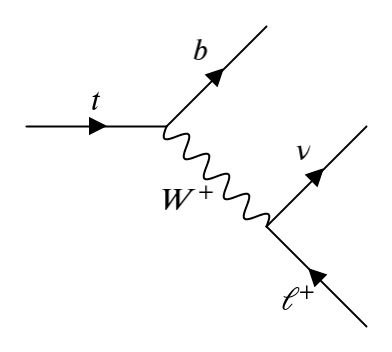
\includegraphics[width=\linewidth]{top1.png}
        \caption{top decay}
        \label{fig:top1}
    \end{subfigure}
    \begin{subfigure}{0.2\linewidth}
        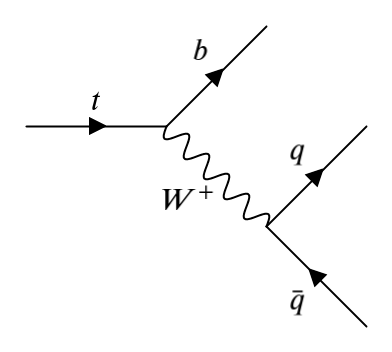
\includegraphics[width=\linewidth]{top2.png}
        \caption{anti-top decay}
        \label{fig:anttop1}
    \end{subfigure}
    \begin{subfigure}{0.2\linewidth}
        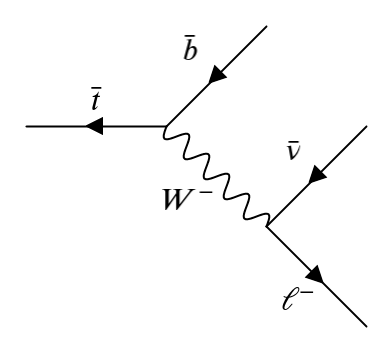
\includegraphics[width=\linewidth]{top3.png}
        \caption{top decay}
        \label{fig:top2}
    \end{subfigure}
    \begin{subfigure}{0.2\linewidth}
        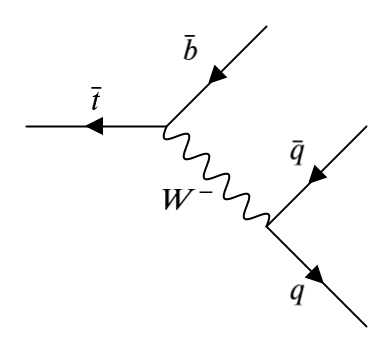
\includegraphics[width=\linewidth]{top4.png}
        \caption{anti-top decay}
        \label{fig:anttop2}
    \end{subfigure}
    \caption{Feynman diagrams of possible (anti-)top decays.}
    \label{fig:decayDiag}
\end{figure}


%-------------------------------------------------------------------------%
\section{The Minimal Supersymmetric Standard Model (MSSM)}
What makes SUSY interesting and an ideal candidate to study phenomena beyond the SM, is the ability to unify all four forces with the potential inclusion of gravity and introducing dark matter candidates. It also solves other problems, for example, why the Higgs mass lighter than the top quark but not other particles. Despite the applicability, SUSY is too generalized and can be depicted as a completely new theory rather than an extension to the SM. The MSSM serves as a bridge between SUSY and the SM by considering it as an \textit{extension} to the SM rather than a completely new theory, making it an ideal model to study. \\

The \textit{symmetry} depicted in MSSM,  is chosen to be the same symmetry group as that of the SM so that it serves as an extension \cite{baer2006weak}. This means that 
%the formalism remains as $SU(3)_c \times SU(2) \times U(1)$, and 
any SUSY transformation would yield the same quantum numbers as that of the SM \cite{aitchison2007supersymmetry}. More generally, the fermions and bosons shown in Tables \ref{tab:SMFerm} and \ref{tab:SMBos} are speculated to have superpartners (or supermultiplet) - the supersymmetric counterparts to each matter and field listed in the Tables \ref{tab:SMFerm} and \ref{tab:SMBos}, as seen in Tables \ref{tab:SUSYspart} and \ref{tab:SUSYinos} respectively. We will refer to these as SUSY particles, or \textit{sparticles}, from hereon. By convention the SM particles and sparticles are distinguished by a tilde, $\Tilde{particle}$.\\

\begin{table}[htbp]
    \centering
    \begin{tabular}{||c|c|c|c||}
    \hline
    & Gen1 & Gen2 & Gen3 \\
    \hline
    & \\[-2.7ex]
    \multirow{2}{1.4cm}{squarks} & $\Tilde{u}$ & $\Tilde{c}$ & \small$\Tilde{t}$ \\
     & $\Tilde{d}$ & $\Tilde{s}$ & $\Tilde{b}$ \\
    \hline
    
    \multirow{2}{1.4cm}{sleptons} & $\Tilde{e}$ & $\Tilde{\mu}$ & $\Tilde{\tau}$ \\
     & $\Tilde{\nu_e}$ & $\Tilde{\nu_\mu}$ & $\Tilde{\nu_\tau}$ \\
    \hline
    \end{tabular}
    \caption{The super-partners of the quarks and leptons in the SM.}
    \label{tab:SUSYspart}
\end{table}

\begin{table}[htbp]
    \centering
    \begin{tabular}{||c|c||}
    \hline 
       Gauginos  & Higgsinos \\
       \hline
        & \\[-2.5ex]
      $\Tilde{g}$, $\Tilde{B}$, $\Tilde{W}$ & $\Tilde{H}$ \\
     \hline
    \end{tabular}
    \caption{The super-partners of the Force carriers in the SM.}
    \label{tab:SUSYinos}
\end{table}

These sparticles have simplistic names, wherein the SM matters will include an ``s" in front of the SM counterpart's name, i.e. \textit{quark} versus \textit{squark} and \textit{leptons} versus \textit{sleptons}. Furthermore, these will turn bosonic (scalar) under a SUSY transformation as depicted in Equation (\ref{eq:states1}) \cite{martin1997supersymmetry}. The gauge and scalar fields in the SM, on the other hand, will turn fermionic (Equation (\ref{eq:states2})) \cite{martin1997supersymmetry}, thus giving rise to the ``-ino" ending to the SM counterpart names, i.e. \textit{gauge bosons} versus \textit{gaugino} and \textit{Higgs} versus \textit{Higgsino}. Note that the neutral component is instead called \textit{Bino} instead of ``Zino" and \textit{Wino} has a neutral component as well.  The Higgsino in SUSY would require two independent components ($\Tilde{H}_u$ and $ \Tilde{H}_d $), unlike SM, due to Yukawa interactions being forbidden with the complex scalar field and its Hermitian conjugate \cite{aitchison2007supersymmetry}. Higgsinos would also have charged and neutral components. This alone shows that Table \ref{tab:SUSYinos} is simplified to match the number of components to Table \ref{tab:SMBos}, where in reality there are a few more extra components already due to complicated theories. \\

The MSSM, therefore, serves as an exact supersymmetric extension to the SM by introducing a \textit{minimum} number of new parameters at just one \cite{aitchison2007supersymmetry}. In other words, the number of new particles introduced is kept at a minimum to serve as a valid model beyond the SM. \par
\begin{align}
     Q\ket{\text{Fermionic}} = \ket{\text{Bosonic}} 
     \label{eq:states1}
     \\
     Q\ket{\text{Bosonic}} = \ket{\text{Fermionic}}
     \label{eq:states2}
\end{align}

However, this symmetry would require that these sparticles have the same mass distributions as their SM counterparts which we know not to be true simply from such particles not being observed in collider experiments. This would imply that the symmetry is broken in an unknown way, allowing these sparticles to acquire masses at a very high mass (energy) scale collider experiments cannot reach yet. MSSM also adds many more free parameters due to its constraints of introducing the minimum number of new particles. This makes things much more sophisticated and difficult to express the correct masses to the new particles exactly. \\

The gauge invariance required in the SM ``accidentally" \cite{martin1997supersymmetry} guarantees the conservation of quantum numbers known as baryon (B) and lepton (L) numbers for all interactions \cite{baer2006weak}. In MSSM, $B$ and $L$ are not necessarily conserved thus not considered as fundamental symmetries nature as there are $B$- and $L$- violating effects strongly constrained by experiment \cite{martin1997supersymmetry}. One can then introduce a globally symmetric and newly conserved quantum number \textit{R-parity} \cite{martin1997supersymmetry, baer2006weak} represented by Equation (\ref{eq:MPrec})
\begin{equation}
    P_R=(-1)^{3(B-L)+2s}
    \label{eq:MPrec}
\end{equation}
where $s$ is the spin of the particle. Different literature may simply denote $P_R$ \cite{martin1997supersymmetry} as $R$ \cite{baer2006weak}. This symmetry conveniently separates SM particles and sparticles in a way that the SM particles have $P_R=+1$ (even R-parity), whereas the sparticles all have $P_R=-1$ (odd R-parity) \cite{martin1997supersymmetry}. In MSSM, the conservation of $R$-parity comes from SUSY events as a pair-produced event \cite{aitchison2007supersymmetry}. \\

%for each particle in MSSM, given by Equation (\ref{eq:MP})
%\begin{equation}
%    P_M=(-1)^{3(B-L)}
%    \label{eq:MP}
%\end{equation}
%where $ P_M = -1 $ for squarks and sleptons, and $  P_M = +1 $ for Higgsinos and gauginos. The principle employed is that the product of $P_M$ for all of the fields in the Lagrangian is +1 for it to be allowed \cite{martin1997supersymmetry}. \\

The MSSM introduces one extra particle known as the lightest supersymmetric particle (LSP) which is stable and neutral, supporting the theoretical properties of a proposed dark matter in cosmology. Analogous to dark matter, a candidate particle is introduced named as \textit{neutralino}. To be precise, there are four possible neutralinos formed by the combination of neutral higgsinos ($\Tilde{H}_u^0$ and $ \Tilde{H}_d^0 $) and neutral gauginos ($\Tilde{B}$ and $\Tilde{W}^0$), denoted as $\Tilde{N}_i$ for $i=1,2,3,4$ \cite{martin1997supersymmetry}. The hierarchy of their mass is $ m_{\Tilde{N}_1} < m_{\Tilde{N}_2} < m_{\Tilde{N}_3} < m_{\Tilde{N}_4}$, where the lightest of the four ($\Tilde{N}_1$) is the prime candidate to be the LSP unless $R$-parity is not conserved \cite{martin1997supersymmetry}. For further information regarding the generation of mass terms and their properties, the reader is referred to SUSY textbooks such as references \cite{martin1997supersymmetry} and \cite{baer2006weak}. \\

The LSP ($\Tilde{N}_1$ sometimes denoted as $\Tilde{\chi}_i^0$) is the only neutralino that cannot decay, whereas other heavier neutralinos may decay via two-body, three-body decays and so on. In collider experiments, the `detection' of the LSP would rely on searching through the missing energies of a SUSY event which is thought to be at the order of $ 2m_{\Tilde{N}_1}$ \cite{aitchison2007supersymmetry}, hence making them difficult to detect.  \\
